\chapter{Theoretical Background}

Motor learning in MR builds on many aspects, eg. suitable technology for MR representations and what perspectives to use. Furthermore, human motor learning must be suitably transfered in the digital world. And eventually, we need to match movements and measure the error correctly to derive adequate from the performance of a learner. In this chapter we take a look into these topics. 

\section{Movements}
\subsection{How do we learn movements}
We learn by mimicking others, follow textual descriptions, videos etc. \todo 
%Beschreiben wie wir generell bewegungen erlernen nicht unbedingt mit bezug auf lernen in MR

\subsection{Movement classification}
For a simplified discussion a classification of movements is provided in the following. There are two important classification schemes. The first one is based on the particular movements performed and are divided into \textit{discrete}, \textit{continuous} and \textit{serial movements}. The second one is based on perceptual attributes of the task and are divided into \textit{open} and \textit{closed skills}. Both classification representing a continuum.

\subsubsection{Discrete, Continuous and Serial Movements}
\begin{figure}
	\centering
	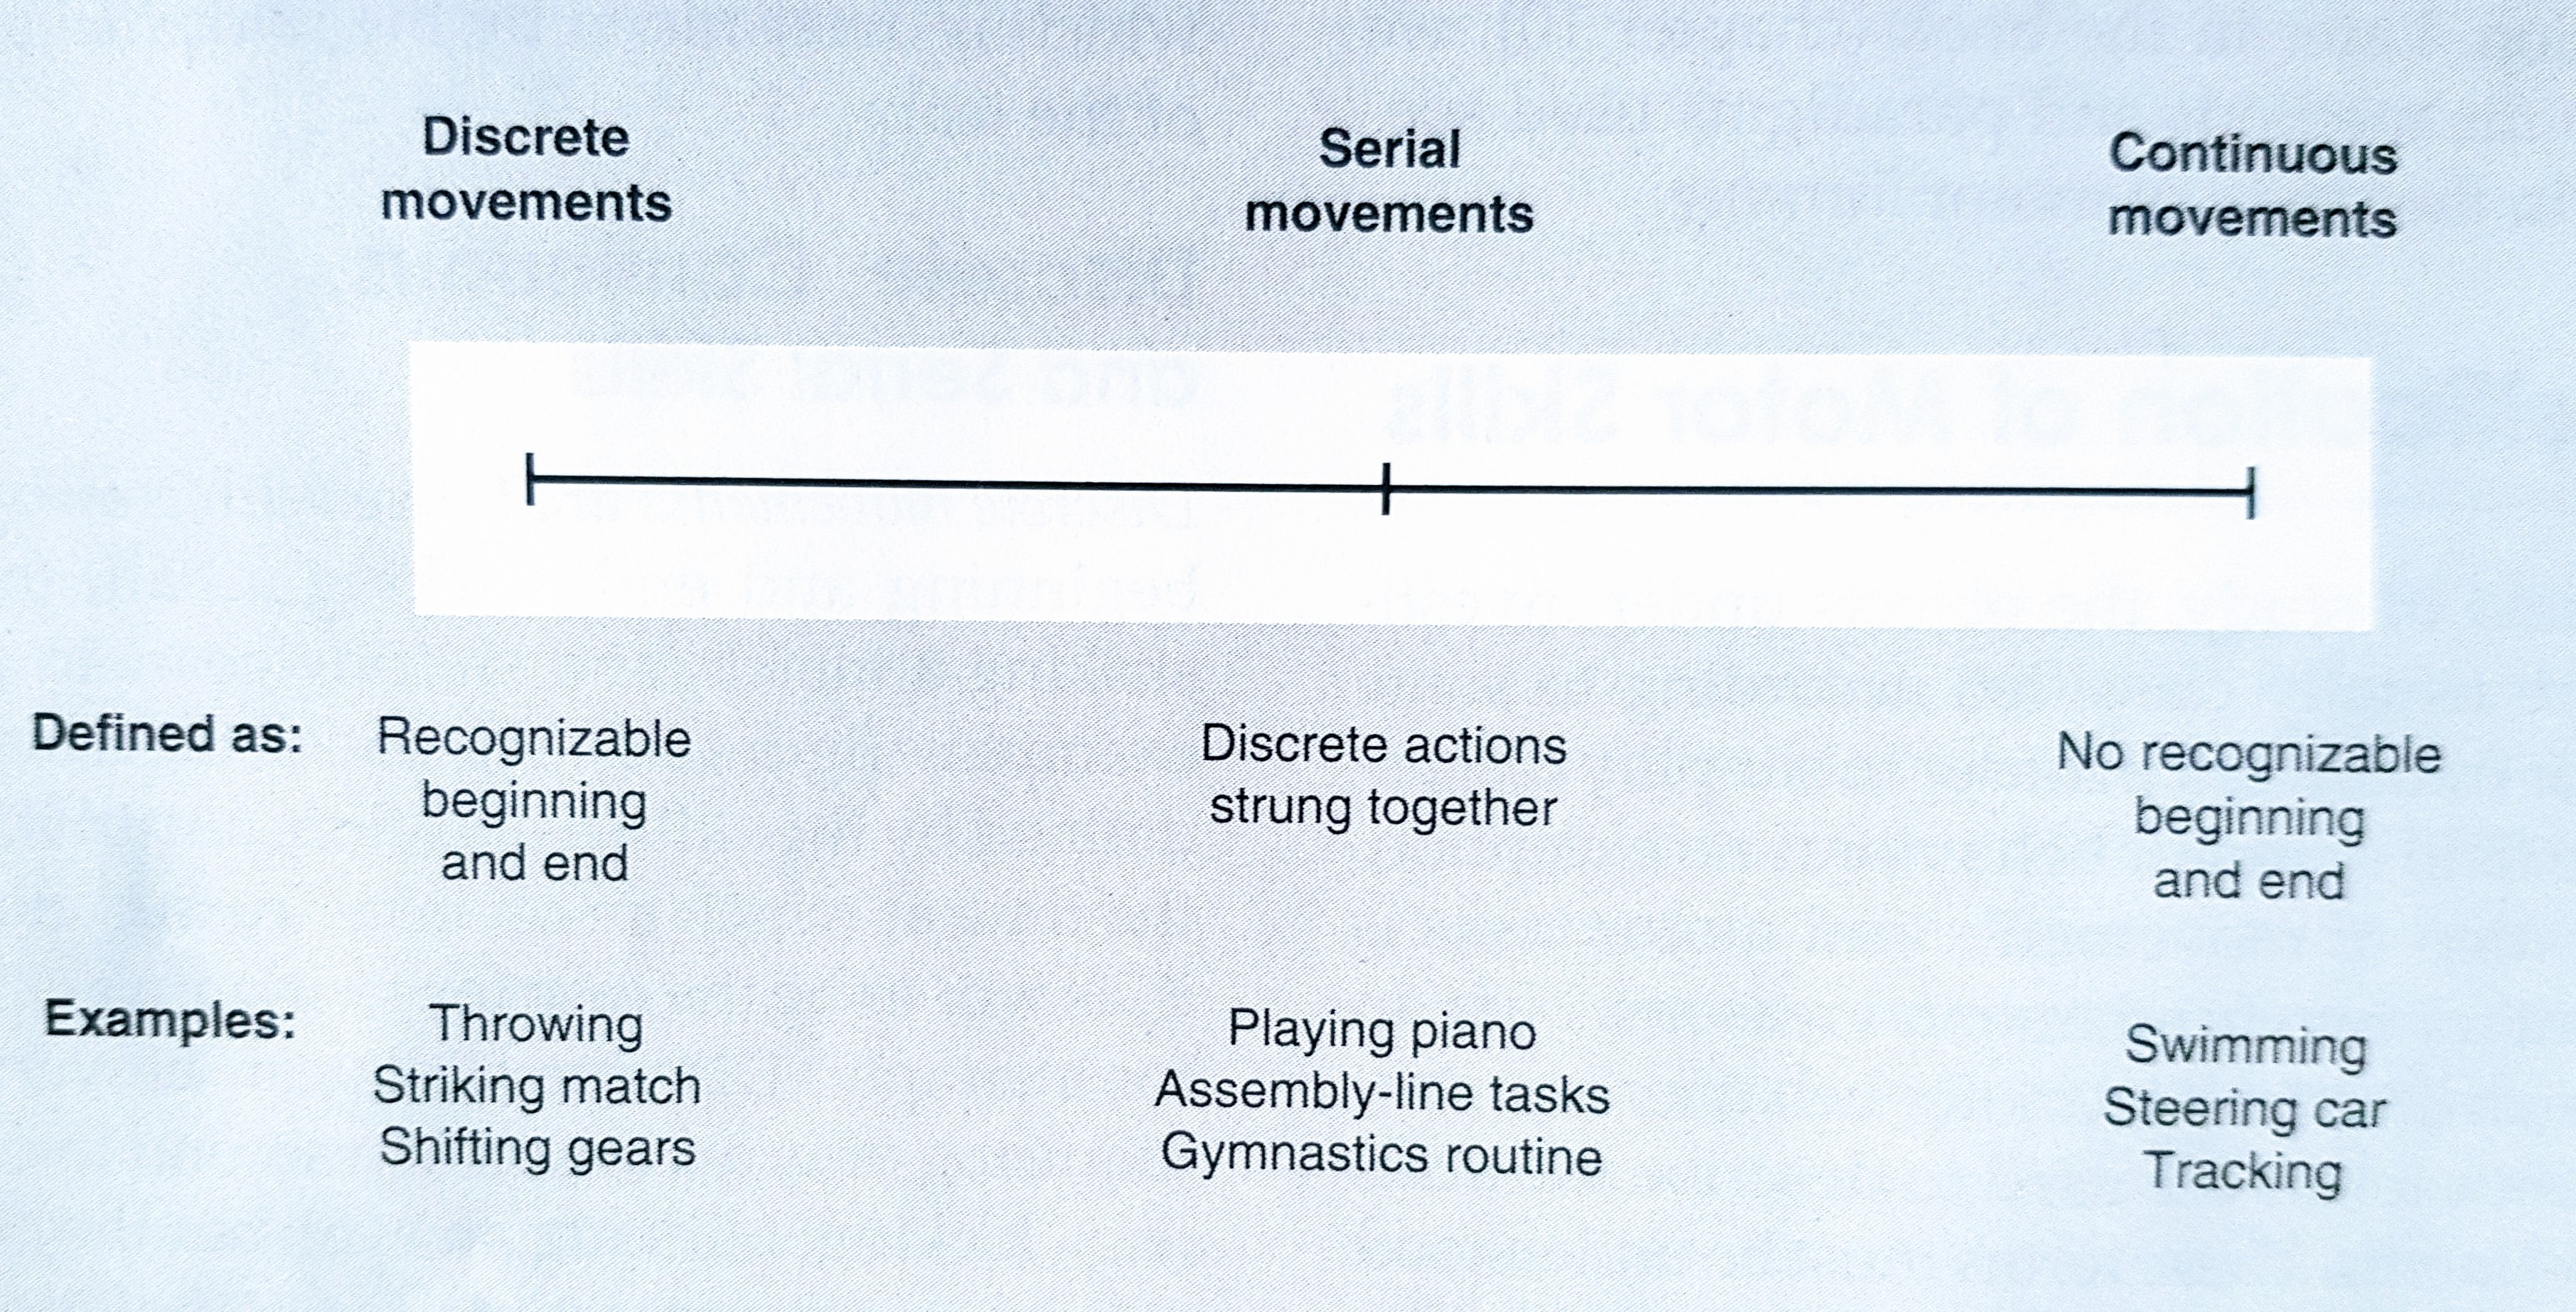
\includegraphics[width=1.0\textwidth]{img/movements_cont.jpg}
	\caption{Continuum of movements buch \cite{Schmidt2011}}
	\label{fig:movements_cont}
\end{figure}
\textit{\textbf{Discrete movements}} are located on the one end of the continuum. These are movements with a recognisable beginning and end. The end of a discrete movement is defined by the task itself and can be very rapid like blinking or longer like making the signing. Examples are kicking a ball, shifting gears in a car or striking a match\\
\textit{\textbf{Continuous movements}} are located on the other end of the continuum. These movements don't have a recognisable start and end, with behaviour continuing till the movement arbitrarily stopped. Continuous tasks tend to be longer than discrete tasks. Examples are swimming, running or steering a car.\\
\textit{\textbf{Serial movements}} are located in the middle part of the continuum. Following the nature of a continuum these movements are neither discrete nor continuous. They can consist of smaller movements tied together. Furthermore, discrete movements can be rather long but are not stopped arbitrarily. Serial tasks can be seen as many discrete tasks strung together and the order (and sometimes timing) is important. Examples are starting a car or preparing and lighting a wood fireplace.

\subsubsection{Open and Closed Skills}
\textit{\textbf{Open skills:}} The environment is constantly, unpredictably changing, so the performer cannot plan his activity effectively in advance. Own movements depend on the environment. For example, if a ice hockey player shoots a shot in ice hockey, his own movement is dependent on the movement of the keeper. Another example is  driving on a free way. The driver needs to adjust his own driving dependent on the behaviour of the other cars. Success in open skills is largely determined by the extend to which a individual can adapt the planned motor behaviour to the changing environment.\\
\textit{\textbf{Closed skills:}} The environment is predictable, mainly because it is stable. This means that the performer can plan his activity in advance. Examples are bowling, archery or singing.
\todo + citations

\begin{figure}
	\centering
	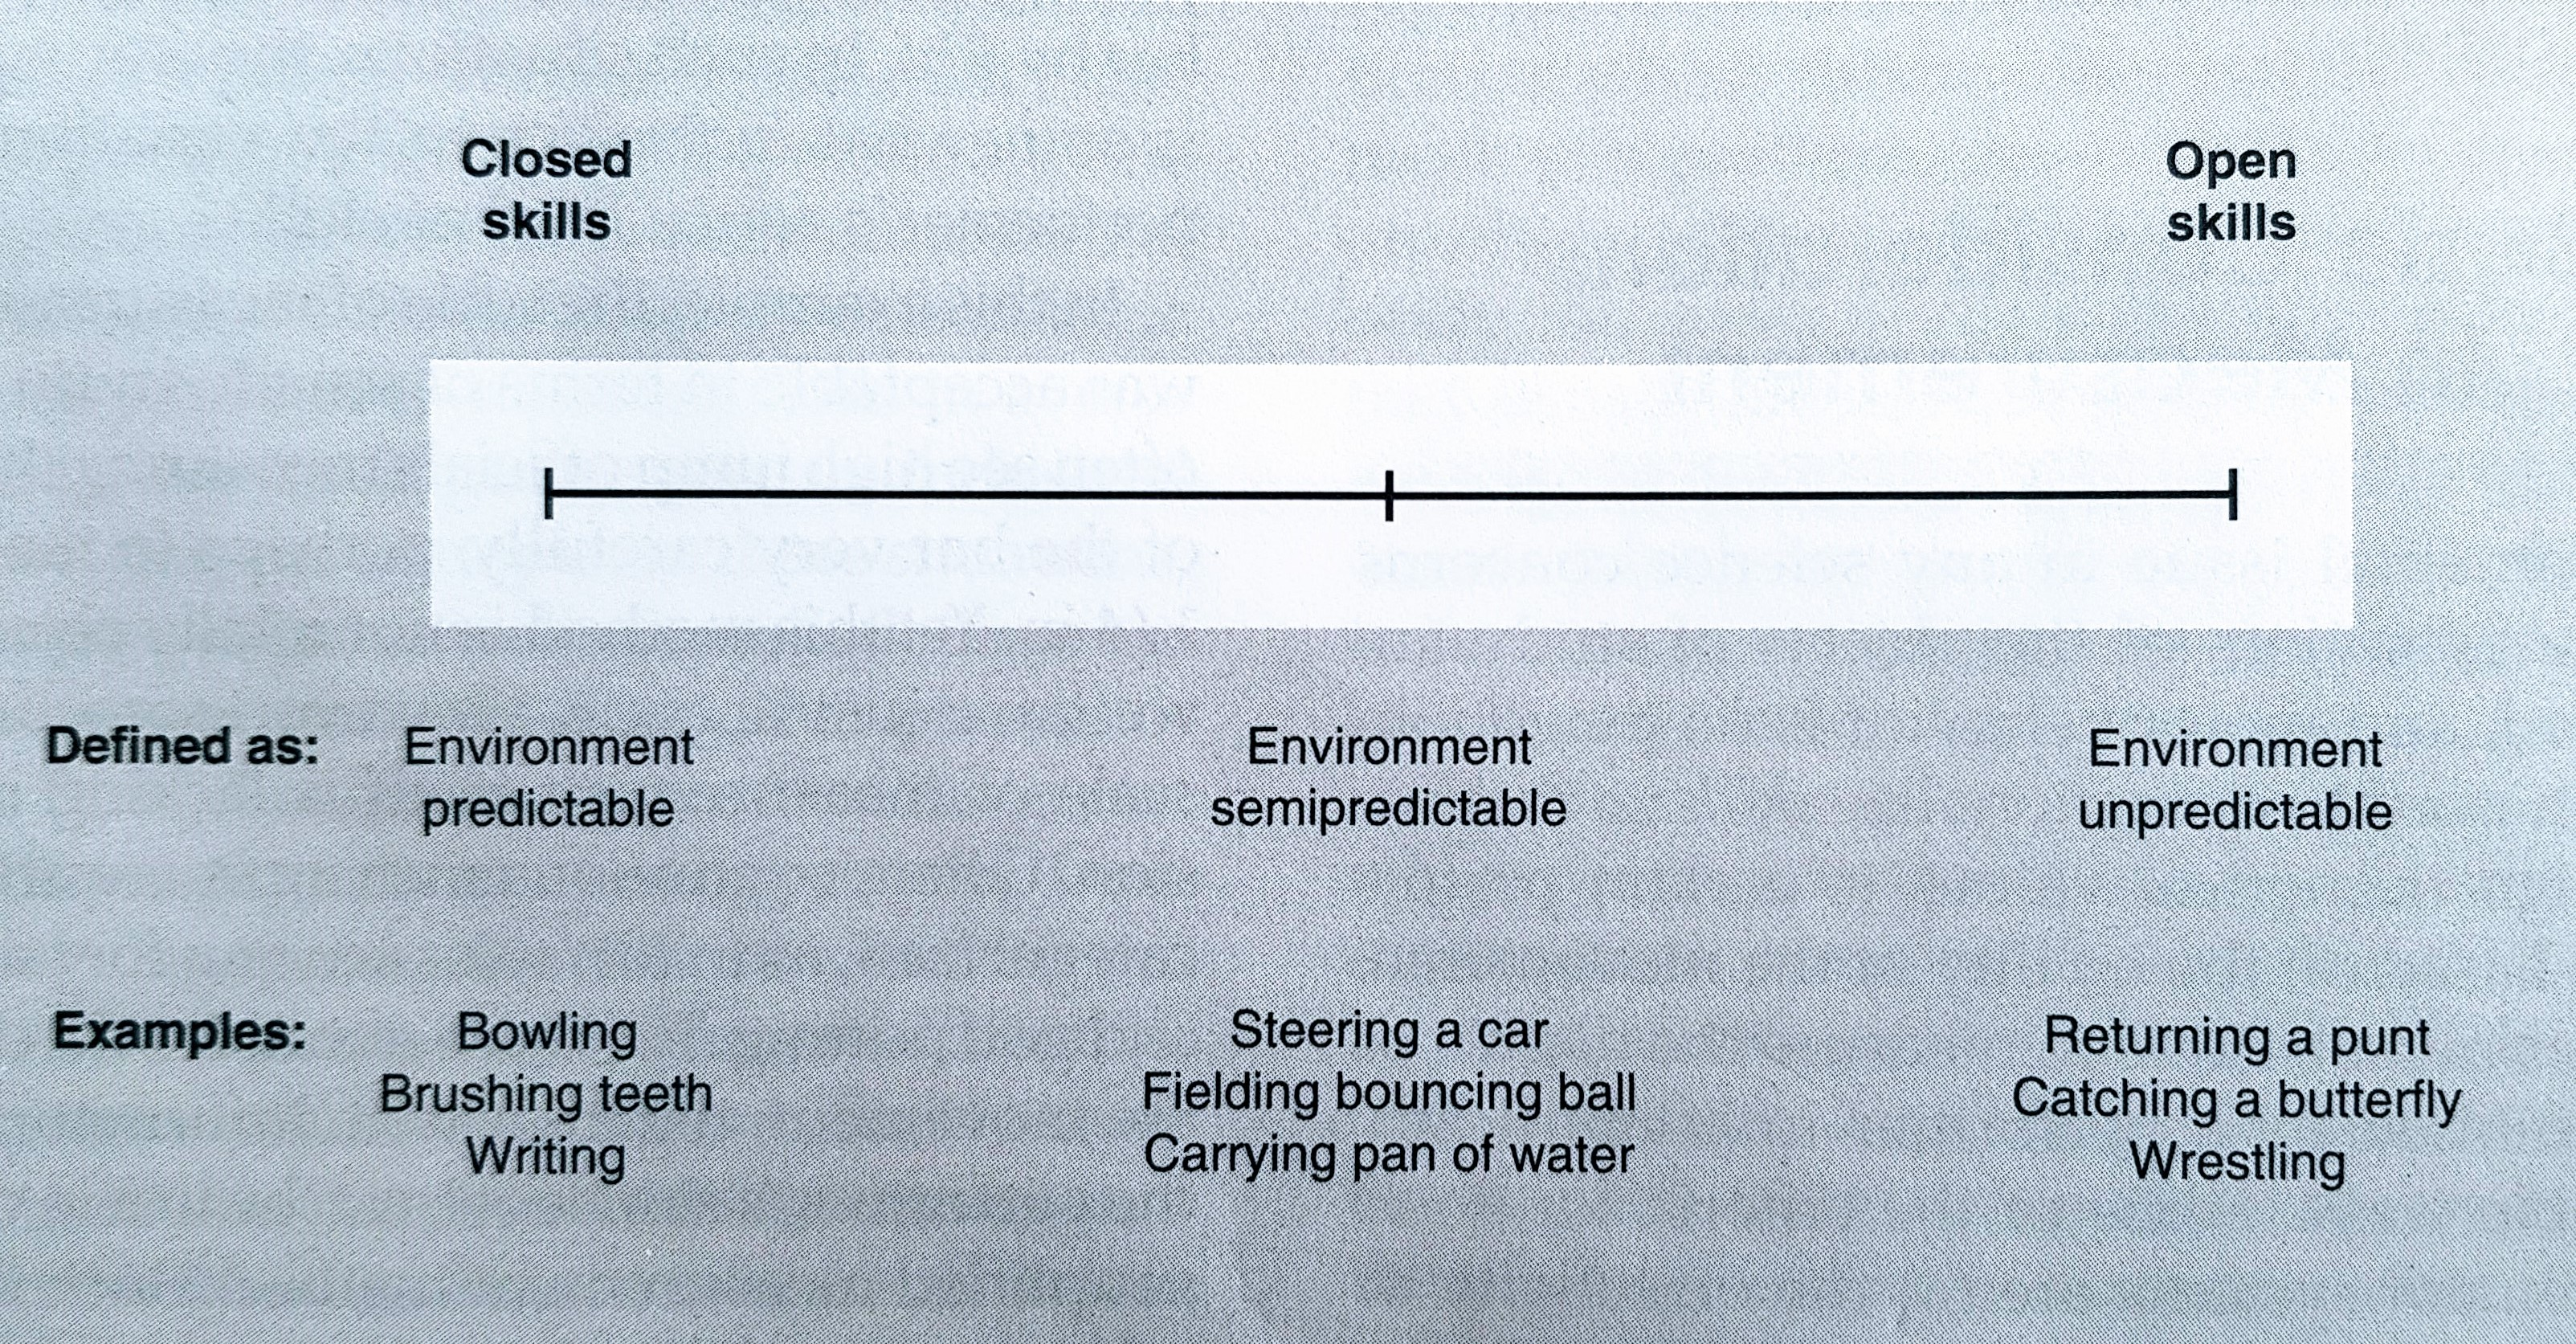
\includegraphics[width=1.0\textwidth]{img/skills_cont.jpg}
	\caption{Continuum of skills \cite{Schmidt2011} \todo seite}
	\label{fig:skills_cont}
\end{figure}
%since open skills  seems to require rapid adaptions to a changing environment and closed skills require a very stable performances in a predictable environment questions are raised about the method of training, do different individuals perform better in in one of these skill classes. to overcome these question the focus of this seminar is on discrete movement tasks and closed skills. $->$ see study \todo + citations

%gespiegelte, ungespiegelt, synchron, asynchron -> max fragen

\subsection{How to quantify movements}
%Wie können bewegungen überhaupt quantifiziert werden
Judging motions and matching them to a given motion is not a trivial task. One approach follows Rudolph von Laban - a professional dancer. Von Laban developed a broadly used dance notation. His work lead to the \textit{Laban Movement Analysis} with which human movements could be quantized.\footnote{Brockhaus, Rudolf Laban. http://www.brockhaus.de/ecs/enzy/article/laban-rudolf (accessed 2018-10-25)} There are four main components to systematically describe movements in the \textit{Laban Movement Analysis}: body, effort, shape and space. Each component can describe movements independently or combined. Hachimura et al. \cite{Hachimura2005} used the methodology  of \textit{Laban Movement Analysis} and adopted it to for digital movements.\\
Yoshimura et al. \cite{Yoshimura2005} followed a similar approach from another dance movement description theory called \textit{furi}. \textit{Furi} is also described by four so called \textit{indices}: \textit{kamae}, \textit{jyu-shin}, \textit{koshi}, \textit{uchiwa}. Yoshimura at all could map these indices to concrete markers on the body of a performer.
%They showed that there was a significant difference between movements by an expert and a beginner.
Qian et al. \cite{GangQian2005} developed a gesture recognition system for performing arts. To match the motions ten body parts were defined: head, torso, upper arms, forearms, upper legs and lower legs. For each body part the Mahalanobis distance is calculated to an ideal point. The Mahalonobis distance describes the distance between point \textit{p} and distribution \textit{D}. Kwon et al. \cite{Kwon2005} \todo 
\begin{itemize}
	\item K. Hachimura, K. Takashina, and M. Yoshimura, “Analysis and
	Evaluation of Dancing Movement Based on LMA,” Proc. IEEE Int’l
	Workshop Robots and Human Interactive Comm., pp. 294-299, 2005.
	\item M. Yoshimura, N. Mine, T. Kai, and L. Yoshimura, “Quantification	of Characteristic Features of Japanese Dance for Individuality Recognition,” Proc. IEEE Int’l Workshop Robot and Human Interactive Comm., pp. 193-199, Sept. 2001.
	\item G. Qian, F. Guo, T. Ingalls, L. Olson, J. James, and T. Rikakis, “A	Gesture-Driven Multimodal Interactive Dance System,” Proc. IEEE	Int’l Conf. Multimedia and Expo (ICME ’04), pp. 1579-1582, June	2004.
	\item D.Y. Kwon and M. Cross, “Combining Body Sensors and Visual
	Sensors for Motion Training,” Proc. ACM SIGCHI, pp. 94-101,	2005.
	\item vr dance trainer
\end{itemize}

\subsection{How to measure movements}
%Welche messmethoden gibt es um bewegungen zu messen
In order to judge if a movement is performed correctly methods need to be applied to measure the error of a performed action. In literature, three main categories are listed: error of a single subject, measures of time and speed and measures of movement magnitude.
\subsubsection{Measures of Error for a Single Subject}
Measures of error for a single subject represent the degree to which the target was not achieved. A target can be to perform an act at a particular time (time stamp), move with a certain force (amount of force) or hit a spatial target (a point in spatial volume). The attribute of the target serves as the variable in question, see braces behind the examples. The error itself describes the distance - in regard to the dimension - from the target. The following list gives an insight to the most important error measures.
\begin{itemize}
	\item \textbf{\textit{Constant Error}} describes the average error between the actual accuracy and the target. Means, in average the performer missed the target by CE.
	\begin{equation}
		CE=\frac{\sum_i(x_i-T)}{n}
	\end{equation}
	\label{eq:constanterror}
	with $x_i$: score, $n$: number of values, $T$: target value.
	\item \textbf{\textit{Variable Error}} measures the inconsistency in movements. The more consistent the movements, the smaller $VE$. $VE$ does not depend on whether or not the subject was close to the target.
	\begin{equation}
		VE=\sqrt{\frac{\sum(x_i-M)^2}{n}}	
	\end{equation}
	\item \textbf{\textit{Total Variability}} describes the total variability around a target. The combination of VE and CE represents the total amount of spread about the target. It is an overall measure how successful was the subject in achieving the target.
	\begin{equation}
		E=VE^2+CE^2=\sqrt{\frac{\sum(x_i-T)^2}{n}}
	\end{equation}
	with $x_i$: score, $n$: number of values, $T$: target value.
	\item \textbf{\textit{absolute error}} is a measure of the overall accuracy in performance.
	\begin{equation}
		AE=\frac{\sum|x_i-T|}{n}
	\end{equation}
	with $x_i$: score, $n$: number of values, $T$: target value.
	\item \textbf{\textit{Absolute Constant Error}} is the absolute value of $CE$. Because of negative and positive values can cancel each other out
	\begin{equation}
		ACE = |CE|
	\end{equation}
\end{itemize}
these measures can be applied to other movements. like pursuit motor: TOT, Mashburn task, stabilometer, two hand coordination task.

\subsubsection{Measures of Time and Speed}
\underline{measures of time and speed}: basic to this idea: performer who can accomplish more in a given amount of time or who can accomplish a given amount of behavior is  more skillfull. time measure:c $\frac{time}{unit}$. speed:$\frac{units}{time}$.\\

\underline{reaction time} (RT): can also be a performance measure. a measure of time from the arrival of a sudden and unanticipated signal to the beginning of the response. 
\subsubsection{Measures of Movement Magnitude}
\underline{movement time (MT):} how long does the movement last. somtimes commbined with RT: response time$=RT+MT$
%i will only describe it if i will use it

\subsection{Movement Classification}
eg. Postural, Transport, Manipulation. p4 in motor learning, principles and practices
\todo after analysis

\section{Mixed Reality}
Mixed reality continuum \cite{Milgram1994} and something about when AR or VR is better.

\begin{figure}
	\centering
	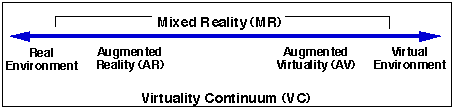
\includegraphics[width=1.0\textwidth]{img/milgram_continuum.png}
	\caption{Mixed reality continuum by Milgram et al. \cite{Milgram1994}}
	\label{fig:ego-exo-cont}
\end{figure}

\section{Perspectives}
Wang and Milgram \cite{Wang2001} describe the perspectives on the centricity continuum see figure \ref{fig:ego-exo-cont}. On the most left hand side of the continuum the egocentric perspective is located. Egocentric means that the anchor of the viewport camera is located inside the object to control - for simplicity, this object in question is referred as avatar. On the left hand side the exocentric perspective is located. This viewport camera is a fixed camera in the scene not to be controllable. The exocentric perspective gives the user the possibility to examine the scene from a bird's-eye view. The movement or angle of the avatar has no influence on the cameras position or angle. So the main difference is the so called tether distance and the degree of freedom of the camera. Milgarm and Wang investigated on tethered cameras and define it as the distance between the avatar and the camera which is following the avatar. This describes the middle part of the continuum. Zero-distance camera describes the egocentric perspective. The longer the tether distance the more the perspective is located on the right of the scale to the exocentric perspective. They also distinguish between dynamic and rigid tethering relation ships. A dynamic tethered camera is controlled by the user in all six dofs (\todo) while a rigid stands like a pole and can only be controlled in 3 dofs. Rigid tethered cameras are common in modern 3rd person computer games.
\begin{figure}
	\centering
		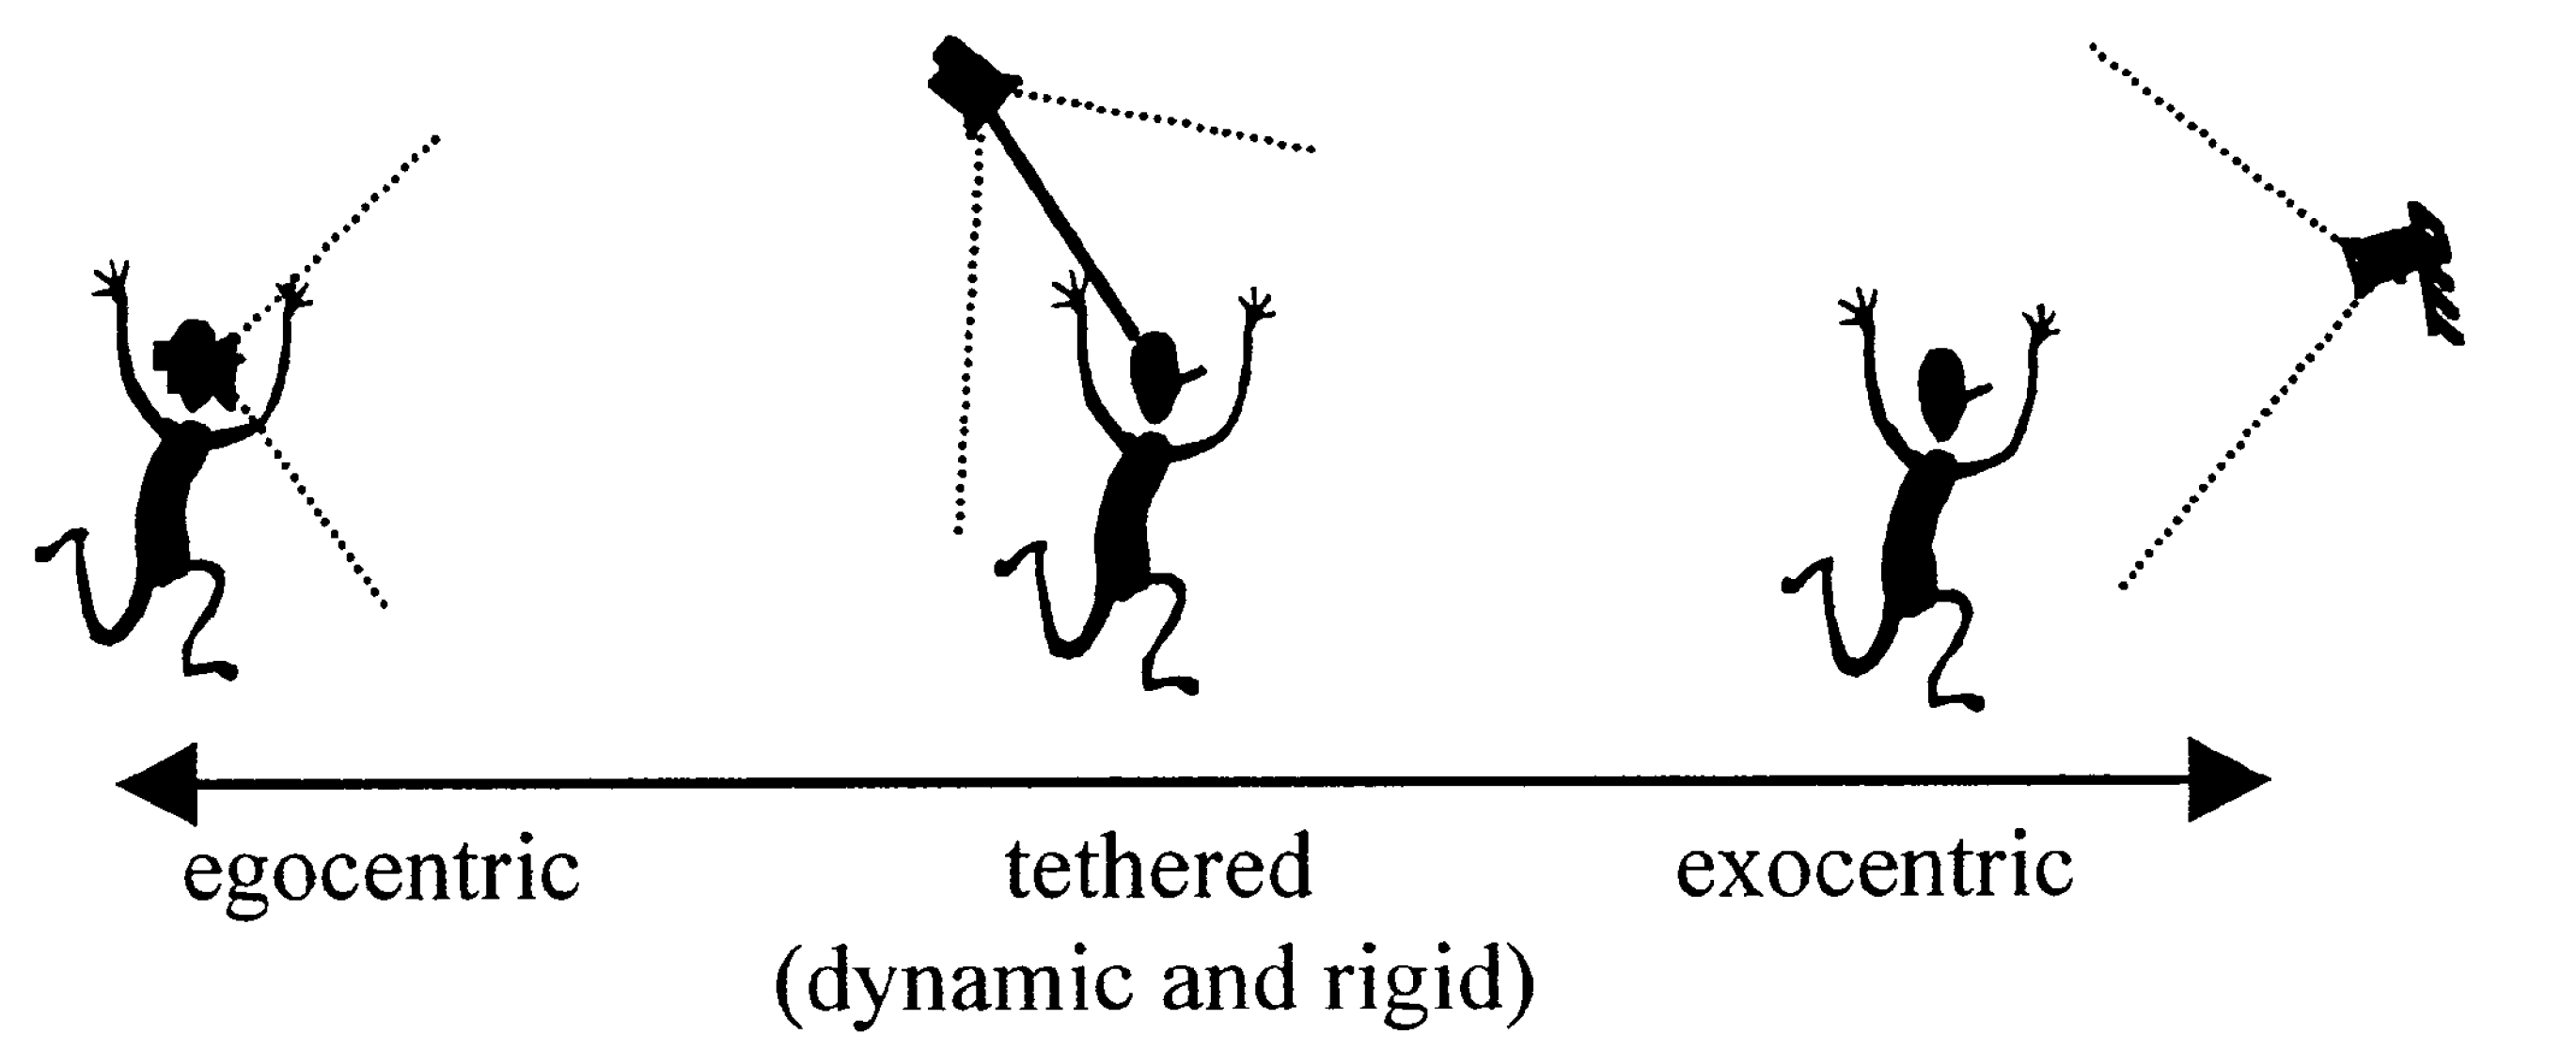
\includegraphics[width=1.0\textwidth]{img/ego_exo_continuum_bigger.PNG}
	\caption{Centricity continuum by Wang and Milgram 2001 \cite{Wang2001}}
	\label{fig:ego-exo-cont}
\end{figure}

\section{VR Technologies}
HMD,3D screens, tablets

\section{Motion Tracking Technologies}
External vs. internal tracking. Drift problem, accuracy

\section{asynchron vs synchron}

\section{Application}
Einsatzmöglichkeiten und MLSF \todo
\begin{itemize}
	\item Theory practical transfere by variation of virtual content
	\item location independet communication and sharing of experience
	\item individual support of reflextion internal
	\item support of reflextion external
\end{itemize}